%================================================================== Logo On/Off
\LogoOff

%==================================================================FRONT PAGE AND TOC
% For article only
\mode<presentation:0>{\thispagestyle{empty}\maketitle}

% For presentation only
\mode<presentation| article:0| handout:0>{
    \begin{frame}<article:0>[label=portada]
    \titlepage
    \end{frame}%Fin del frame
}

% For handout only
\mode<handout>{
  \begin{frame}[label=portada]
    \maketitle
  \end{frame}
}

%% TABLE OF CONTENTS
\begin{frame}[label=toc]
    \mode<article:0>{\frametitle{Contents}}
    \mode<presentation>{\small}
    \tableofcontents%[hidesubsections]
\end{frame}

%%==================================================================S
\section[Objetivo]{Objetivo}
%%==================================================================F
\begin{frame}
  \frametitle{Objetivo}
  \begin{enumerate}
    \item Es necesario extraer información de la nube de puntos: terreno,
      no-terreno.
    \item Paso imprescindible para la generación de DTM
    \item Clasificación en diferentes categorías:
      \begin{itemize}
        \item Terreno
        \item Edificio
        \item Vegetación
        \item Pasos elevados, etc\ldots
      \end{itemize}
    \item Las idea subyacente son también aplicables otras técnicas como TLS,
      pero con características diferentes (densidad).
  \end{enumerate}
\end{frame}
%%==================================================================S
\section{Definición de filtro}
%%==================================================================F
\begin{frame}[label=filter_def]
    \frametitle{Filtros ALS}
    %\onslide<1->\begin{beamerboxesrounded}[shadow=true]{Definición: \emph{Nube de puntos LiDAR}}
    % Es un conjunto de puntos tridimensionales con un atributo asociado: 
    % $V = \left\lbrace \mathbf{p}=\left(\mathbf{x},c\right) | x \in \mathbb{R}^3, c \in \mathbb{N} \right\rbrace$
    %\end{beamerboxesrounded}
    \begin{beamerboxesrounded}[shadow=true]{Definición: \emph{Clasificación}}
      Dada una nube de puntos,$V = \left\lbrace \mathbf{p}=\left(\mathbf{x},c\right) 
      \left| x \in \mathbb{R}^3, c \in \mathbb{N} \right. \right\rbrace $, se 
      puede definir como \alert{\emph{clasificación}} a la función $f: \mathbf{x} \to c$ 
      que a cada punto tridimensional, $\mathbf{x}$, le asigna su atributo, $c$.
    \end{beamerboxesrounded}

    {El problema formal de clasificar se restringe a encontrar la función $f$ tal que asigna:
    \begin{itemize}
      \item \alert{1}, si el punto pertenece a un \alert{objeto}
      \item \alert{0}, si el punto pertenece al \alert{terreno}
    \end{itemize}}

    \begin{beamerboxesrounded}[shadow=true]{Definición: \emph{Filtrar}}
     Consiste en \alert{eliminar} los puntos de $V$ con atributo igual 1 (objeto) y dejar los clasificados como 0 (terreno).
    \end{beamerboxesrounded}
\end{frame}
%%==================================================================S
\section{Tipos de clasificaciones}
%%==================================================================F
\begin{frame}
    \frametitle{Tipos de clasificaciones}
    \begin{enumerate}
        \item Morfológicos
        \item Densificación progresiva
        \item Basado en superficies
        \item Segmentación y \emph{clustering}
        \item Estudio de pendientes (splines)
    \end{enumerate}
\end{frame}
%%==================================================================Sb
\subsection{Morfológicos}
%%==================================================================F
\begin{frame}
  \frametitle{Filtros morfológicos}
  \begin{enumerate}
    \item \alert{Morfología}: Conjunto de métodos del análisis de imágenes que
      dan una descripción cuantitativa de estructuras geométricas.
    \item Existen dos operadores básicos: \alert{Erosión} y \alert{dilatación}.
    \item Ayudan a simplificar la estructura de una superficie basándose en un
      cierto elemento estructural.
    \item Combinaciones de ambos:
      \begin{itemize}
        \item \alert{apertura}: erosión $\to$ dilatación
        \item \alert{clausura}: dilatación $\to$ erosión
        \item Ayudan a determina el máximo y el mínimo basándose en un cierto elemento.
      \end{itemize}
    \item Normalmente los algoritmos se aplican a los puntos 
    \item La morfología matemática tiene sus orígenes en estructuras ráster:
      ayudan a agilizar los cálculos
  \end{enumerate}
\end{frame}
%%==================================================================F
\begin{frame}
  \frametitle{Filtros morfológicos: Linderberger (1993)}
  \begin{enumerate}
    \item Utiliza como elemento estructural una ventana móvil que desplaza 
      a lo largo de todos los puntos
    \item La ventana se puede adaptar según la densidad de puntos
    \item Las operaciones de apertura y clausura generan la superficie superior
      e inferior que representan los puntos en la ventana
    \item La erosión y la dilatación determinan el punto central de la ventana
      según el punto más bajo y más alto en ella
    \item La superficie más baja es considerada como el DTM y se usa para
      filtrar los puntos según una tolerancia en altura
  \end{enumerate}
\end{frame}
%%==================================================================F
\begin{frame}
  \frametitle{Filtros morfológicos}
  \begin{center}
    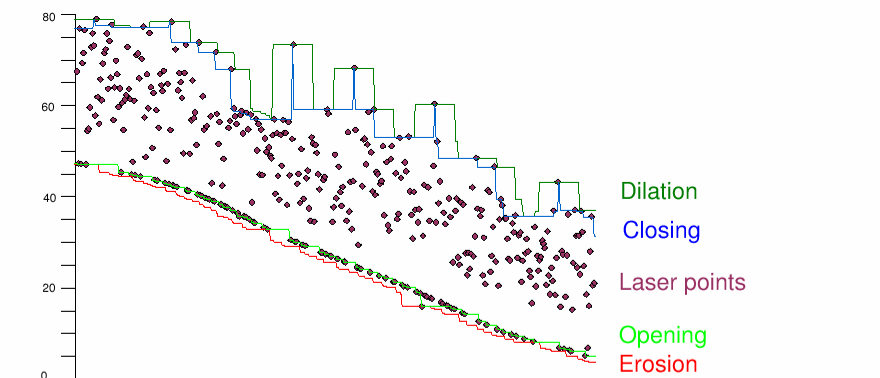
\includegraphics[height=0.70\textheight]{images/morfologia}
  \end{center}
\end{frame}
%%==================================================================F
\begin{frame}
  \frametitle{Filtros morfológicos: Vosselman (2000)}
  \begin{enumerate}
    \item El elemento estructural es una función que describe la diferencia de
      altura máxima admisible según la distancia al punto
      \begin{itemize}
        \item Generalmente un círculo
        \item La función se puede definir a partir de la pendiente máxima del
          escenario
        \item Mediante áreas de entrenamiento se puede llegar a un elemento
          óptimo que minimice los errores por comisión y omisión
      \end{itemize}
    \item Se posiciona el elemento estructural en cada punto 
    \item Si alguna de las alturas de los puntos en el ámbito del elemento 
      estructural es mayor que la máxima altura permitida, el punto es 
      considerado como no-terreno.
  \end{enumerate}
\end{frame}
%%==================================================================F
\begin{frame}
  \frametitle{Filtros morfológicos: Vosselman (2000)}
  \begin{center}
    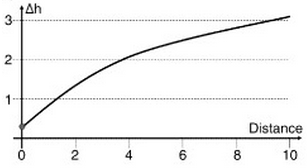
\includegraphics[height=0.70\textheight]{images/morph_element}
  \end{center}
\end{frame}
%%==================================================================F
\begin{frame}
  \frametitle{Filtros morfológicos: Sithole (2001)}
  \begin{enumerate}
    \item Basado en Vosselman (2000)
    \item Utiliza una función adaptativa según en la pendiente del terreno 
      para determinar la diferencia de altura admitida
    \item Necesita un DTM inicial cuyas celdas toman el valor de la menor altura
      entre todos los puntos del píxel
  \end{enumerate}
\end{frame}
%%==================================================================Sb
\subsection{Densificación progresiva}
%%==================================================================F
\begin{frame}
  \frametitle{Filtros de densificación progresiva}
  \begin{enumerate}
    \item Triangulación progresiva de un TIN 
    \item Empiezan con un pequeño subconjunto de puntos de la nube: pre-clasificación del terreno
    \item Incrementan de manera iterativa la cantidad de información para
      clasificar todo la nube paso a paso.
    \item Para incrementar siguen varios criterios: ángulos y altura respecto a
      los triángulos del TIN
      \begin{itemize}
        \item Hansen y Vögtle (1999)
        \item Axelsson (2000)
        \item Sohn y Dowman (2002)
      \end{itemize}
  \end{enumerate}
\end{frame}
%%==================================================================F
\begin{frame}
  \frametitle{Filtros de densificación progresiva: Axelsson (2000)}
  \begin{enumerate}
    \item El conjunto inicial de puntos se genera a partir de una compartición
      en bloques y eligiendo, para cada bloque, el punto con altura más baja
    \item Este conjunto se triangula generando una aproximación del terreno
    \item Se añade un punto más al modelo si se verifica cierto criterio
      \begin{itemize}
        \item Los ángulos $\alpha_i = \widehat{PA_i}, i=1,2,3$ entre la cara del
          triángulo y las líneas que unen los tres puntos $A_i$ son más pequeños
          que ciertos valores dados
      \end{itemize}
    \item El proceso se repite hasta que:
      \begin{itemize}
        \item no se pueden añadir más puntos al TIN, o
        \item si se alcanza cierta densidad puntual: los lados de todos los
          triángulos son más pequeños que un umbral
      \end{itemize}
  \end{enumerate}
\end{frame}
%%==================================================================F
\begin{frame}
  \frametitle{Filtros de densificación progresiva: Hansen y Vögtle (1999)}
  \begin{enumerate}
    \item El conjunto inicial de puntos se genera como la parte más baja de
      cierre convexo de los puntos de la nube
    \item Este conjunto se triangula generando una aproximación del terreno
    \item Se añade un punto más al modelo si se verifica cierto criterio
      \begin{itemize}
        \item La diferencia de alturas entre el punto candidato y la superficie
          del triángulo
      \end{itemize}
    \item El proceso se repite hasta que:
      \begin{itemize}
        \item no se pueden añadir más puntos al TIN, o
        \item si se alcanza cierta densidad puntual: los lados de todos los
          triángulos son más pequeños que un humbral
      \end{itemize}
  \end{enumerate}
\end{frame}
%%==================================================================F
\begin{frame}
  \frametitle{Filtros de densificación progresiva: Sohn y Dowman (2002)}
  \begin{enumerate}
    \item El conjunto inicial de puntos se genera mediante:
      \begin{itemize}
        \item los puntos más bajo de las cuatro esquinas del área a filtrar
        \item Se densifica el conjunto inicial añadiendo el punto más bajo 
          en cada triángulo hasta que no se pueden añadir más
      \end{itemize}
    \item Se añade un punto más al modelo si está en un \emph{buffer} respecto a
      la superficie actual y si verifica un criterio de \emph{Minimum
      Description Length} (\alert{MDL})
      \begin{itemize}
        \item Minimiza la cantidad necesaria de puntos para describir la
          superficie
      \end{itemize}
  \end{enumerate}
\end{frame}
%%==================================================================Sb
\subsection{Superficies}
%%==================================================================F
\begin{frame}
  \frametitle{Filtros basados en superficies}
  \begin{enumerate}
    \item Utilizan una reconstrucción de superficies de referencia
    \item Similares a la densificación progresiva
    \item Asumen que todos los puntos de la superficie pertenecen al terreno 
    \item Progresivamente eliminan puntos que no se ajustan al modelo de tereno
  \end{enumerate}
  \begin{center}
    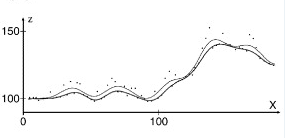
\includegraphics[height=0.40\textheight]{images/surfbased_filter}
  \end{center}
\end{frame}
%%==================================================================F
%\begin{frame}
%  \frametitle{Filtros basados en superficies}
%  \begin{center}
%    \includegraphics[height=0.50\textheight]{images/surfbase_filter}
%  \end{center}
%\end{frame}
%%==================================================================F
\begin{frame}
  \frametitle{Filtros basados en superficies: Kraus y Pfeifer (1998)}
  \begin{enumerate}
    \item Basado en una \alert{interpolación robusta}: trata de determinar un peso 
      $p_i \in [0;1]$ para cada punto $P_i$ de modo que la superficie 
      modelada represente el terreno
      \begin{enumerate}
        \item Interpolación de la superficie considerando los pesos. Al inicio
          $p_i = 1$
        \item Cálculo de valores $f_i$: distancia entre la superficie y el punto $P_i$
        \item Cálculo de un nuevo peso $p_i$ en base a los $f_i$
        \item Estos pasos se repiten hasta:
          \begin{itemize}
            \item Llegar a una superficie estable (los pesos permanecen estables)
            \item Alcanzar un número máximo de repeticiones
          \end{itemize}
      \end{enumerate}
    \item Integra el filtrado y la generación del DTM en el mismo proceso
    \item Los puntos son clasificados como terreno y no-terreno basándose en un
      umbral para la diferencia de altura entre el punto y la superficie
  \end{enumerate}
\end{frame}
%%==================================================================F
\begin{frame}
  \frametitle{Filtros basados en superficies: Elmqvist \emph{et al.} (2001)}
  \begin{enumerate}
    \item La superficie se determina minimizando una función
      \alert{\emph{energía}} en la que entran en juego dos parámetros:
      \begin{itemize}
        \item \alert{Rigidez} o fuerza interna:
        \item Las observaciones o fuerza externa que obliga a la superficie a
          pasar por ellas
      \end{itemize}
     \item La superficie inicial es horizontal y está por debajo de todos los
       puntos
     \item La ``fuerza'' de los puntos se aplica de manera iterativa
       $\Rightarrow$ La superficie se deforma hacia los puntos
     \item La deformación está restringida por la rigidez de la superficie
     \item Asegura la poca influencia de puntos objetos y su aproximación al
       terreno
     \item La clasificación se realiza con una banda de tolerancia alrededor de
       la superficie final
  \end{enumerate}
\end{frame}
%%==================================================================Sb
\subsection{Segmentación}
%%==================================================================F
\begin{frame}
  \frametitle{Filtros de segmentación}
  \begin{enumerate}
    \item Clasifican \alert{segmentos} enteros de puntos: conjuntos de puntos
      vecinos con propiedades similares
    \item Intentan evitar el problema de puntos individuales mal clasificados
    \item Hay dos pasos básicos
      \begin{itemize}
        \item Generar por agregación segmentos de puntos
        \item Clasificar dichos segmentos
      \end{itemize}
    \item Se pueden elegir varios algoritmos para cada paso
  \end{enumerate}
\end{frame}
%%==================================================================F
\begin{frame}
  \frametitle{Filtros de segmentación}
  \begin{enumerate}
    \item Se utilizan técnicas de \alert{crecimiento de regiones}
    \item Se agrupan puntos vecinos con propiedades similares dentro de un
      umbral: altura, vector normal, etc,\ldots
    \item La segmentación se puede hacer en el espacio objeto:
      \alert{segmentación}
    \item o en el espacio de las características: \alert{\emph{clustering}}
  \end{enumerate}
\end{frame}
%%==================================================================F
\begin{frame}
  \frametitle{Filtros de segmentación}
  \begin{center}
    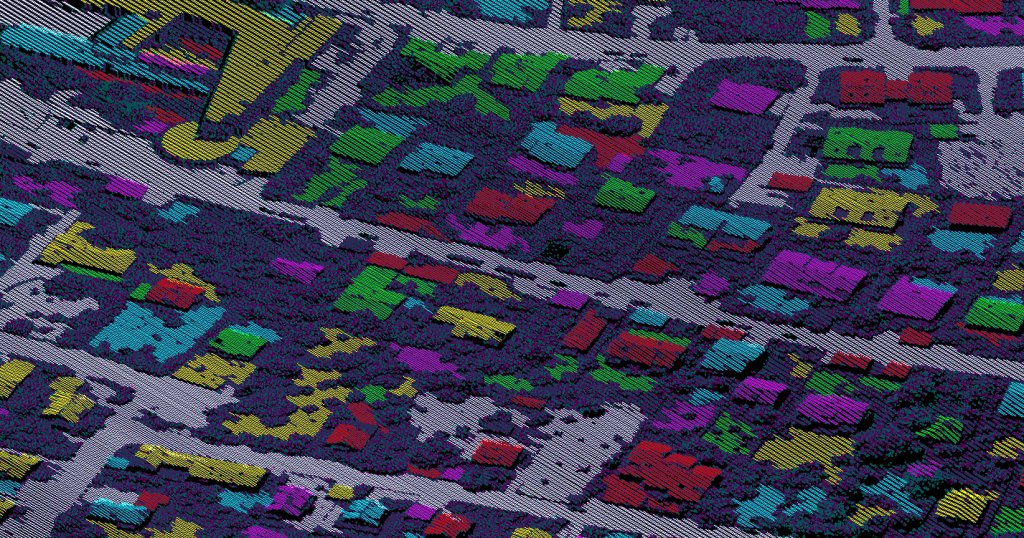
\includegraphics[height=0.70\textheight]{images/clustering}
  \end{center}
\end{frame}
%%==================================================================F
\begin{frame}
  \frametitle{Sithole (2005) y Sithole y Vosselman(2005)}
  \begin{enumerate}
    \item Utilizan los últimos impulsos 
    \item Metodología basada en la intersección de perfiles
      \begin{itemize}
        \item La nube es dividida en diferentes perfiles y los puntos son unidos
          por segmentos siguiendo ciertos criterios
        \item Los segmentos se hallan agrupando los segmentos de los perfiles
      \end{itemize}
    \item La clasificación se basa las relaciones de vecindad de los segmentos
    \item Durante el proceso global se utilizan diferentes criterios para hallar
      puentes, micro y macro objetos y objetos artificiales o naturales
  \end{enumerate}
\end{frame}
%%==================================================================F
\begin{frame}
  \frametitle{Tovari y Pfeifer (2005)}
  \begin{enumerate}
    \item La segmentación se basa en algoritmos de \alert{\emph{region growing}}
    \item Empezando por un punto, se añaden puntos con características
      similares:
      \begin{itemize}
        \item Similitud entre los vectores normales
        \item Proximidad espacial
      \end{itemize}
    \item Después de la segmentación se sigue un filtrado basado en superficies
      mediante una técnica de interpolación robusta
  \end{enumerate}
\end{frame}
%%==================================================================S
\section{Comparación de filtros}
%%==================================================================F
\begin{frame}
  \frametitle{Comparación de filtros}
    \begin{itemize}
      \item Estudio del rendimiento de los 8 filtros distintos 
      \item Auspiciado por el \emph{International Society of Photogrammetry and
        Remote Sensing} (\alert{ISPRS})
      \item Estudio cualitativo y cuantitativo
    \end{itemize}
\end{frame}
%%==================================================================F
\begin{frame}
  \frametitle{Resultados}
  \begin{enumerate}
    \item Todos los filtros funcionan correctamente con escenarios poco exigentes
      \begin{itemize}
        \item Poca o nula pendiente, y extensas zonas de terreno
        \item Pequeños edificios
        \item Vegetación dispersa
      \end{itemize}
    \item Mayores problemas en zonas con:
      \begin{itemize}
        \item Edificios voluminosos con escasa extensión de terreno
        \item Parches de terreno a diferentes alturas o con alturas variables
      \end{itemize}
    \item Mejores prestaciones: \alert{densificación progresiva} y los basados
      en la \alert{determinación de superficies}
    \item Los más desarrollados: \alert{segmentación y clustering}
    \item \alert{Combinación} de varios algoritmos e \emph{inputs} distintos
  \end{enumerate}
\end{frame}
%%==================================================================F
\begin{frame}
  \frametitle{Automatización Vs Manual}
  \begin{enumerate}
    \item Comparados con la fotogrametría, los filtros son procesos \alert{automáticos}
    \item Todavía no se ha encontrado un filtro completamente automático y
      \alert{universal}
    \item \alert{Necesaria} una revisión y edición manual (cercados, umbrales\ldots)
        \begin{center}
        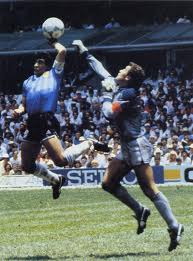
\includegraphics[height=0.60\textheight]{images/mano_dios}
        \end{center}
      \begin{itemize}
        \item Zonas urbanas 
        \item \alert{Innecesaria en zonas rurales}
        \item Puentes y pasos elevados
        \item Algoritmos basados en relaciones geométricas de puntos vecinos
        \item El terreno no puede ser identificado por escasez de puntos
      \end{itemize}
    \item Fuentes de datos adicionales pueden disminuir la revisión
      \begin{itemize}
        \item Delimitación de edificios
        \item Contexto de terreno local
        \item Información radiométrica: \alert{externa} o la \alert{devuelta por
          el láser}
      \end{itemize}
  \end{enumerate}
\end{frame}
%%==================================================================FIN
\begin{frame}
 \titlepage
\end{frame}
